\documentclass{article}
\usepackage[utf8]{inputenc}
\usepackage{mathtools}
\begin{document}
The first step in classifying leaves is extracting utilizable information from the processed image, this is called feature extraction. This procedure tries to find informative values in the image and converts them into a feature vector. To assist the feature extractor the image is first converted to a greyscale. This is done to reduce the dimensionality of the RGB-image from three dimensions (Red Green and Blue), to one dimension. This significantly reduces the processing cost and therefore speeds up the process. The parameters used for the weighted greyscale conversion are $Y = 0.299 * R + 0.587 * G+0.114 * B$. This are the values provided by the openCV library, a open-source computer vision library. After this a mask is applied to inform the feature extractor of the relevant part of the image. This mask is a inverted threshold to zero mask, this means that every pixel with a greyscale above a threshold is set to a greyscale of 0 (black). This threshold, established empirically, was set to 200. After this preprocessing the image is ready for the feature extractor. As mentioned in the introduction, the feature extraction algorithm applied in this research is the Scale-invariant feature transform algorithm, or in short: SIFT. This algorithm was chosen for its ability to swiftly localize keypoints at areas with a high variation, while being scale- and rotation invariant. This invariance is important for the classification of leaves because of the various ways photos can be taken by the users. Also SIFT proves to be a proper algorithm for different viewpoints and varying illumination. To acquire keypoints SIFT uses Difference of Gaussians, DoG finds points by subtracting Gaussian blurred versions of the image from each other, this is done at various scales. This finds local extrema (maxima or minima) in the image, the keypoints. The Difference of Gaussians is calculated by the substraction of the image by the convolution of the image with the Gaussian of variance. 
\delta DoG 
=
I*\frac{1}{\sigma_1\sqrt{2\pi}} \, e^{-(x^2)/(2\sigma^2)}-I*\frac{1}{\sigma\sqrt{2\pi}} \, e^{-(x^2)/(2\sigma^2)}. 
This gives the keypoints depicted in \textit{figure 1}. 
\begin{figure}[p]
    \centering
    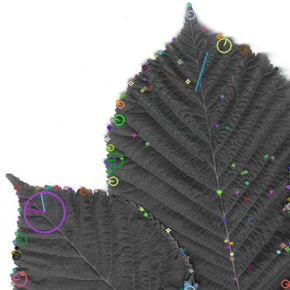
\includegraphics[width=0.8\textwidth]{keypoints.png}
    \caption{Keypoints found by the SIFT algorithm}
    \label{fig:flowchart}
\end{figure}


\begin{figure}[p]
    \centering
    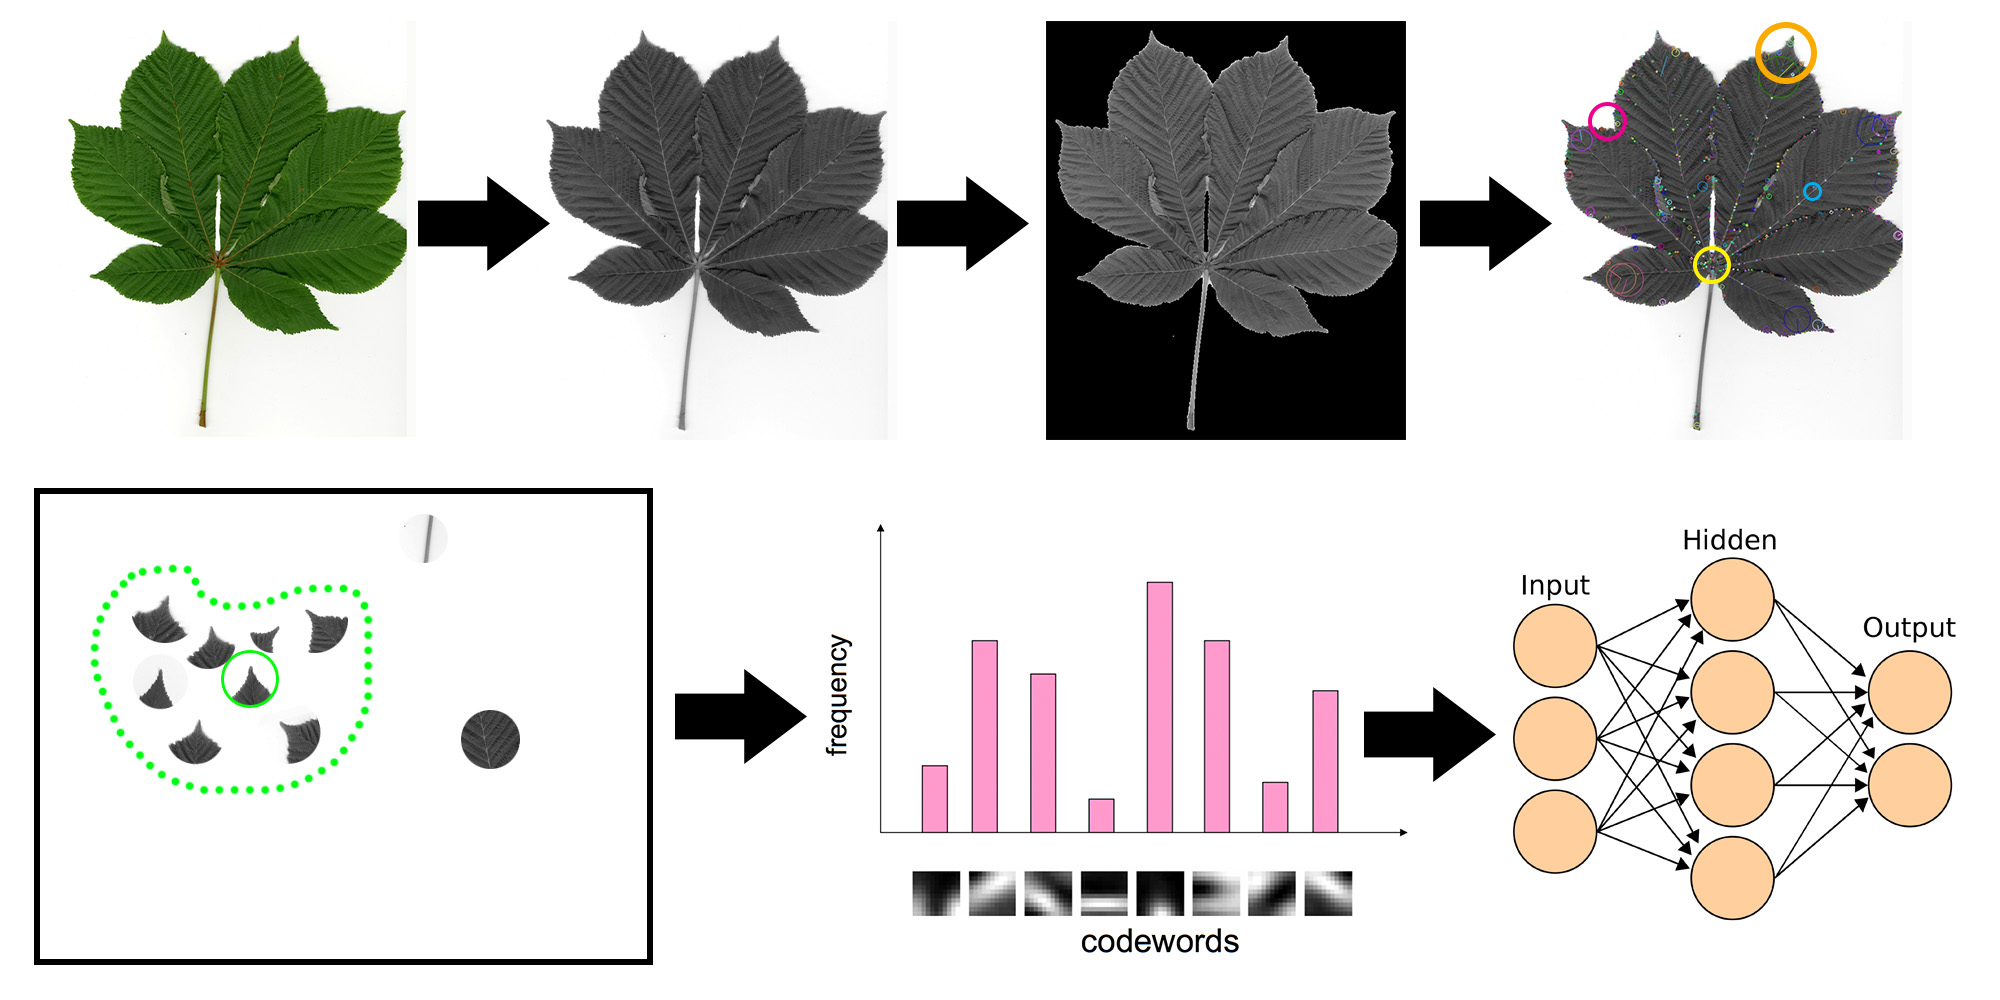
\includegraphics[width=0.8\textwidth]{flowchart.jpg}
    \caption{The classification procedure}
    \label{fig:flowchart}
\end{figure}
\end{document}